\documentclass{article}

% you could use a pre-print version if you want if you don't submit it.
\usepackage{neurips_2019}
\usepackage[utf8]{inputenc}
\usepackage[T1]{fontenc}
\usepackage{hyperref}
\usepackage{url}
\usepackage{booktabs}
\usepackage{amsfonts}
\usepackage{nicefrac}
\usepackage{microtype}
\usepackage{algorithm}
\usepackage{algorithmic}
\usepackage{amsmath}
\usepackage[pdftex]{graphicx}

\title{Unsupervised Creation of Robust Environment Representations for Reinforcement Learning}

\author{}

% Only 8 pages of content are allowed. Additional pages must contain only references.
% fix hyphenation with \-
\begin{document}

\maketitle

% The abstract must be limited to one paragraph.
\begin{abstract}
Reinforcement learning (RL) methods traditionally have suffered from large sample complexities, which reduces their widespread effectiveness.
This is particularly true for the beginning stages of deep RL methods, where the methods must learn what the objects in an environment are in addition to what actions to take.
We aim to improve the sample complexity of deep RL methods by disentangling these two tasks, using unsupervised learning methods to complete the first task.
In particular, we propose a method that embeds learned environmental representations into a Deep Q-Network (DQN), so that the DQN does not have to learn the environment itself.
Specifically, we provide a Rainbow DQN with robust environment representations of Atari video games created through a conditional variational ladder autoencoder with coordinate convolutions.
\end{abstract}

% All headings should be lower case (except for first word and proper nouns.
\section{Introduction}

Reinforcement learning (RL) is a popular area of current research across various fields, including psychology, neuroscience and computer science \cite{kaelbling:reinforcement}.
RL methods train autonomous agents to choose actions that maximize an aggregate reward.
These methods learn through trial and error and consequently are subject to scalability issues.
In particular, they struggle with memory and computational complexity  \cite{arulkumaran:survey}.

Even when these algorithms are scalable, they may have a large sample complexity.
For example, Lake et al. describe a Deep Q-Network (DQN) that was able to achieve human-level performance on some Atari video games, but it took about 500 times more experience for the algorithm to learn to play the games as compared to human subjects \cite{lake:building}.
The drastic difference was even more pronounced in the early training stages as humans had basic knowledge of the video game environments that the DQN did not have.

We aim to improve the sample efficiency of RL algorithms by embedding in them representations of their environment (created  through unsupervised learning methods).
In particular, we create robust representations of Atari video game states through the use of a conditional variational ladder autoencoder with coordinate convolutions.
We then concatenate these compressed representations onto the states in a Rainbow DQN.

The main contributions of this paper are as follows:

\begin{enumerate}
    \item We create robust representations of the Atari game environment. 
    \item We improve the sample efficiency of Rainbow.
    \item We successfully embed unsupervised learning into reinforcement learning.
\end{enumerate}

\section{Preliminaries}

\subsection{Autoencoders}

An \emph{autoencoder} is an unsupervised neural network that attempts to reconstruct its input. 
The network can be seen as having two parts, an encoder function $f(\cdot)$ and a decoder function $g(\cdot)$.
The encoder takes the input $\textbf{x}$ and embeds it into a compressed space, often referred to as the \emph{latent space representation}, $\textbf{z}=f(\textbf{x})$.
The decoder takes this representation and attempts to construct the original input $\textbf{\~x}=g(\textbf{z})$.
In other words, the goal of the autoencoder is to learn $f(\cdot)$ and $g(\cdot)$ so that
$g(f(\textbf{x}))=\textbf{x}$.
It learns $f$ and $g$ by minimizing a loss function between $\textbf{x}$ and $\textbf{\~x}$.
A commonly used loss function for autoencoders is mean-squared error.

A \emph{variational autoencoder} (VAE) forces $f$ to produce a latent representation $\textbf{z}$ that follows a standard Gaussian distribution \cite{kingma:auto-encoding}.
It does this by having the encoder map to a vector of means $\pmb{\mu}$ and vector of standard deviations $\pmb{\sigma}$.
It then draws samples from these vectors, resulting in the latent representation
$\textbf{z} \sim \mathcal{N}(\pmb{\mu}, \pmb{\sigma})$.
A latent loss, the Kullback-Liebler (KL) divergence between the latent space and standard Gaussian distributions, is added to the overall loss of the autoencoder.

A \emph{variational ladder autoencoder} (VLAE) defines a joint distribution of latent representations $p(\textbf{z}_1, ..., \textbf{z}_L)$, where $L$ is the number of representations \cite{zhao:learning}.
Each $\textbf{z}_i$ is the resulting encoding of a network $f_i$.
Each $f_i$ has a progressively deeper structure, leading to the varying levels of abstraction for the $\textbf{z}_i$'s.
These networks are constructed in a ladder-like fashion by having the input to each network $f_i$ be the last layer of the previous network (before it maps to $\pmb{\mu}_i$ and $\pmb{\sigma}_i$).
In the case of $f_1$, the network encodes the input image.
As the network is variational, each $\textbf{z}_i$ is drawn from the Gaussian distribution
$\textbf{z}_i \sim \mathcal{N}(\pmb{\mu}_i, \pmb{\sigma}_i).$
The input of the model is then reconstructed using a ladder of decoder networks, where each $g_i$ inputs the concatenation of $\textbf{z}_i$ and the output of the previous decoder $\textbf{\~z}_{i+1}$
$$ \textbf{\~z}_i = g_i(\textbf{z}_i^\frown\textbf{\~z}_{i+1}).$$
In the case of the first decoder $g_L$, it only takes as input $\textbf{z}_L$.
The last decoder $g_1$ reconstructs the original image.
The loss of the VLAE is the exact same as that of a normal VAE, where the latent representation is defined to be the concatenation of each $\textbf{z}_i$,
$$\textbf{z} = \textbf{z}_1^\frown\cdots^\frown\textbf{z}_i^\frown\cdots^\frown\textbf{z}_L.$$

\emph{Conditional VAEs} (CVAEs) are used to model multi-modal distributions \cite{sohn:learning}.
In particular, they condition specific layers of a VAE on a random variable, often a class.
This conditioning of layers on a random variable has been applied to other types of generative networks.
As an example of this, the \emph{conditional instance normalization} method was developed for style transfer networks \cite{dumoulin:alearned}.
After normalization, this method shifts and scales each network layer $\textbf{h}$
$$\textbf{h} = \pmb{\gamma}_c (\frac{\textbf{h} - \pmb{\mu}}{\pmb{\sigma}}) + \pmb{\beta}_c$$
with separate shift $\pmb{\beta}$ and scale $\pmb{\gamma}$ parameters for each class $c$.

\emph{Coordinate convolutions} (CoordConvs) add coordinate information to convolutions in order to make the transform between high-level spatial latents and pixels easier to learn \cite{liu:anIntriguing}.
It does this by concatenating two channels to a convolution's input.
The first channel contains the $x$-value of each coordinate while the second has the $y$-value.
In other words, the first channel's first row is filled with zeros, the second with ones, etc.
While the second channel's first column is filled with zeros, the second with ones, etc.
The convolution can then decide whether to use this spatial information, or discard it to preserve translational invariance.

\subsection{Q-learning models}

\emph{Q-learning} is a RL method that learns a probability distribution over actions given states, or a policy $\pi$.
The policy is learned through the optimal action-value function
\begin{equation}
\label{action_value}
% Use mathbb fonts throughout
Q^\pi (s_t, a_t) = \mathbb{E}_{\pi}[R_t| s_t, a_t ], 
\end{equation}
where $s_t$ represents the current state, $a_t$ the proposed action, $R_t = \sum_{k=0}^\infty \lambda_{t+1}^k r_{t+k+1}$ is the future discounted cumulative reward,  $r_t$ the reward given at time $t$, and $\lambda_t$ the discount factor.
Models are episodic in practice, so $\lambda_t$ is a constant $\lambda\in [0, 1]$ through all time except for after the ending time $T$, where $\lambda_{t>T}=0$.
$R_t$ is discounted  by $\lambda_{t+1}$ to place heavier interest on more immediate rewards.
The \emph{Q-value} is the action $a_t$ that maximizes the result of Equation \ref{action_value}.
The optimal action-value function follows an identity called the Bellman Equation
\begin{equation}
\label{bellman}
Q^\pi (s_t, a_t) = \mathbb{E}_{s'} [r_{t+1} + \lambda \max_{a'} Q^\pi (s',a')|s_t, a_t].
\end{equation}
The expectation is taken over all the possible states to model the states stochastically.

A \emph{Deep Q-Network} (DQN) was the first model to combine neural networks and reinforcement learning \cite{mnih:human-level}.
Neural networks are often described as function approximators, and in this case a Q-network is a function approximator for discovering the Q-values.
The algorithm uniformly samples a mini-batch of transitions (actions with corresponding states and rewards) from the network's replay memory.
Each transition can be seen as a state in a Markov decision process.
These states are fed iteratively through a Bellman equation update
\begin{equation}
\label{bellman_update}
Q_{i+1} (s_t, a_t) = \mathbb{E}_{s'} [r_{t+1} + \lambda \max_{a'} Q_i (s',a')|s_t, a_t]
\end{equation}
resulting in the policy at each state $\pi_i$ converging to the best policy $\pi$.

A \emph{Rainbow DQN} is an extension of the DQN that incorporates several different improvements upon the algorithm \cite{hessel-rainbow}.
These improvements include decomposing the max operation in the target into action selection and action evaluation to reduce overestimation, prioritized experience replay, and using stochastic layers for exploration ~\cite{van-hasselt:double,schaul:prioritized,fortunato:noisy}.

\section{Related work}

Previous research into improving the sample efficiency of RL methods has often involved transfer learning.
In their papers, Taylor et al. survey and analyze transfer learning in RL contexts \cite{taylor:transfer,taylor:introduction}.
They find that there has been transfer success in the algorithms learning navigation and robot soccer keepaway.
For example, Zhang et al. used RL to teach a robot to navigate a maze \cite{zhang:deep}.
They were able to transfer knowledge from previously mastered mazes to new ones.
Another approach was taken by Moreno et al.
They attempted to embed prior knowledge into the algorithm by restricting its exploration space \cite{moreno:using}.

More specific to the learning of Atari games, Parisotto et al. used an actor-critic method to train an agent to simultaneously learn on a variety of tasks and then generalize what it has learned to other tasks \cite{parisotto:actor}.
They found that their pre-learning methods led to significant speed up in their deep Q-network learning to play 3/7 Atari games that they tested it on.
They attributed the speed up of two of these games (Breakout and Pinball) to the fact that pre-learning was done on a similar game (Pong). 
Chaplot et al. repeated their results in 3D video game environments \cite{chaplot:complex}.

While the above-mentioned research transfers knowledge from one RL method to another trained on a different task, we want to transfer knowledge from an unsupervised method.
Although there has been recent research in combining unsupervised and RL methods, it focuses mainly on methods in the two fields that could be deemed equivalent.
For example, Pfau and Vinyals successfully used a generative adversarial network (GAN) as an actor-critic method where the actor cannot effect the reward  \cite{pfau:connecting}.
Similarly, Fin et al. showed that GANs and some Inverse RL methods are equivalent \cite{finn:connection}.
In contrast to these papers combining unsupervised and reinforcement learning by showing their equivalence in certain situations, we aim to use them in tandem, including their inherent differences.

\section{Methods}

\subsection{Conditional VLAE with CoordConv}

To create our learned representations, we used a VLAE.
We decided to use this model as Zhao et al. showed that it excels at finding disentangled representations \cite{zhao:learning}.
Additionally, we wanted to use its capabilities to model various levels of abstraction.
As we are testing in an Atari video game environment, we made the VLAE conditional to better model the different games.
We made it conditional by using conditional instance normalization on each layer in the VLAE.
Additionally, we replaced each convolutional layer with a CoordConv layer.
We did this to lessen the mode collapse of the placement of objects in the VLAE reconstructions.

We trained the VLAE on randomized screenshots from 10 Atari games,\footnote{Air Raid, Atlantis, Gravitar, Name This Game, River Raid, Seaquest, Solaris, Space Invaders, Time Pilot, and Zaxxon.}  obtained by simulating their respective video game environments and taking random actions.
Random reconstructions of the VLAE can be seen in Figure \ref{fig:vlae}.
Parameters for our implementation, along with ablation studies on the VLAE can be found in Appendix A.

% Figure captions should be lower case (except first word and proper nouns).
\begin{figure}
  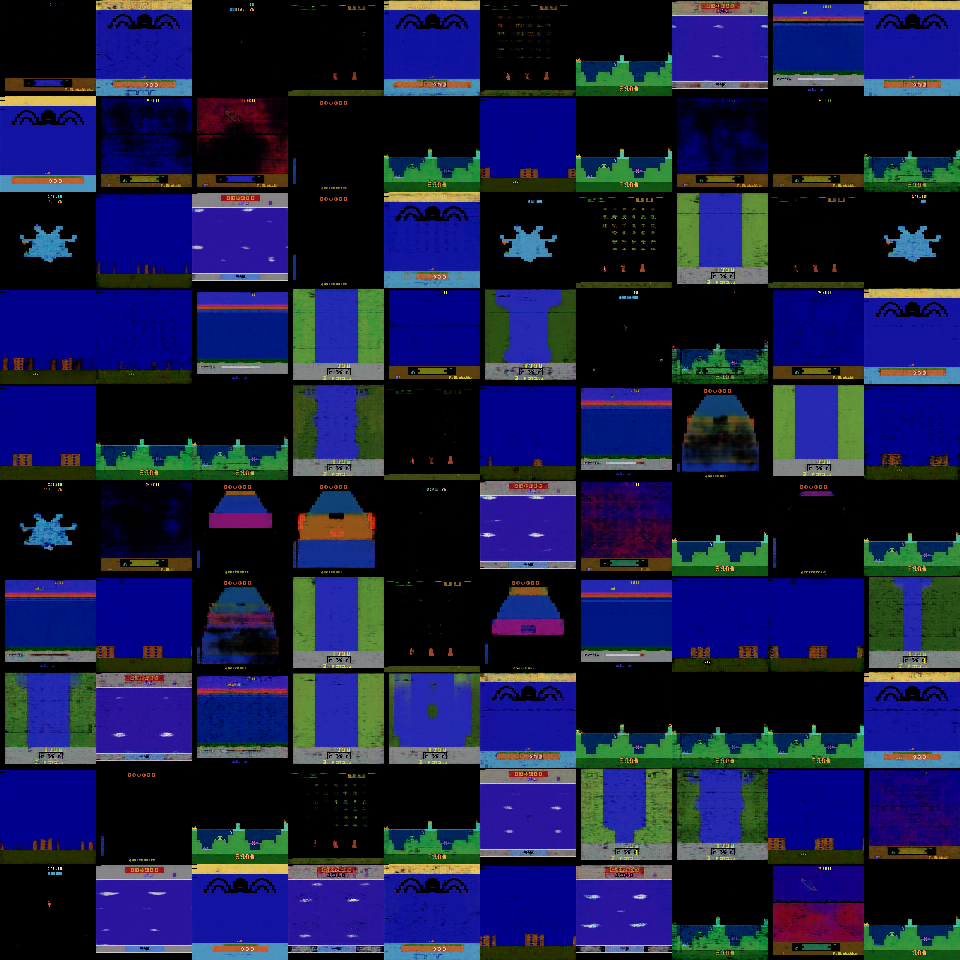
\includegraphics[width=0.8\linewidth]{current.png}
  \caption{Random reconstructions of Atari games using the trained VLAE.}
  \label{fig:vlae}
\end{figure}

\subsection{Rainbow evaluation}

We incorporate the VLAE into Rainbow when it is feeding the transitions (states, actions, and rewards) into the replay memory.
Specifically, we embed each state through the VLAE and concatenate it to the bottom of the state.
When testing on a class that the VLAE has never seen, we pass in a random class into the conditional invariance normalization.
We hypothesize that this added information about the object representations will help Rainbow to be more sample efficient in the early stages.

\section{Results}

\begin{figure}
  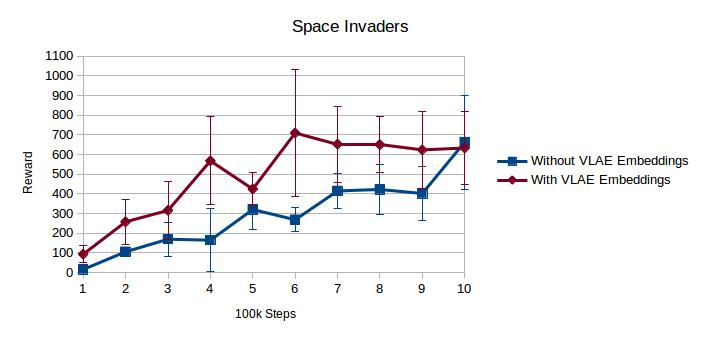
\includegraphics[width=0.8\linewidth]{space_invaders.jpg}
  \caption{The average reward (taken over 10 game simulations) of Rainbow with and without the VLAE embeddings for Space Invaders.}
  \label{fig:spaceinvaders}
\end{figure}

\begin{figure}
  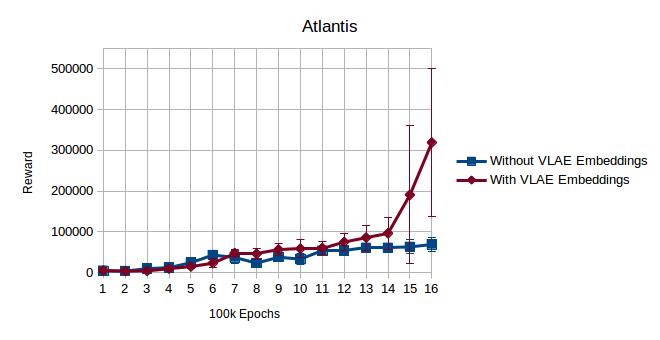
\includegraphics[width=0.8\linewidth]{atlantis.jpg}
  \caption{The average reward (taken over 10 game simulations) of Rainbow with and without the VLAE embeddings for Atlantis.}
  \label{fig:atlantis}
\end{figure}

\begin{figure}
  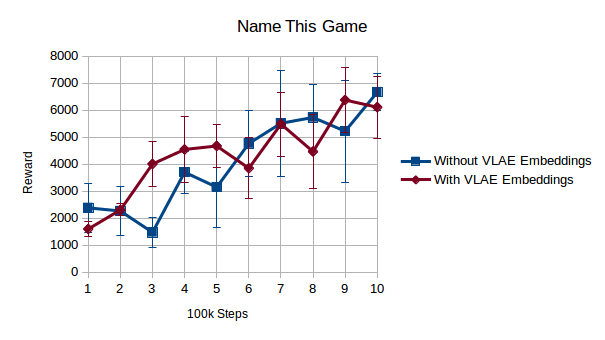
\includegraphics[width=0.8\linewidth]{name_this_game.png}
  \caption{The average reward (taken over 10 game simulations) of Rainbow with and without the VLAE embeddings for Name This Game.}
  \label{fig:name_this_game}
\end{figure}

\begin{figure}
  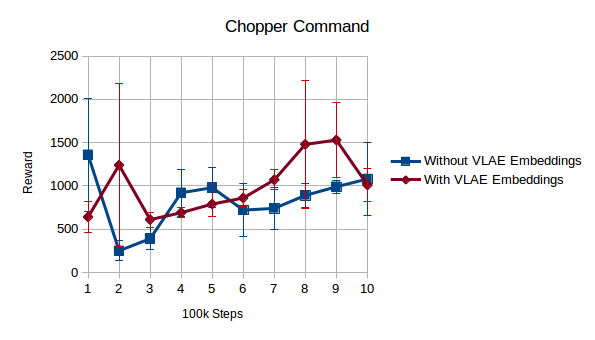
\includegraphics[width=0.8\linewidth]{chopper_command.png}
  \caption{The average reward (taken over 10 game simulations) of Rainbow with and without the VLAE embeddings for Chopper Command.}
  \label{fig:chopper_command}
\end{figure}

\begin{figure}
  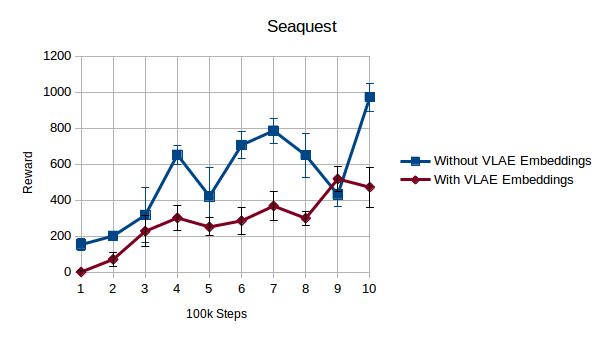
\includegraphics[width=0.8\linewidth]{seaquest.png}
  \caption{The average reward (taken over 10 game simulations) of Rainbow with and without the VLAE embeddings for Seaquest.}
  \label{fig:seaquest}
\end{figure}

We ran Rainbow with the VLAE embeddings on Atlantis, Name This Game, Seaquest, Space Invaders and Chopper Command. 
Notice that we did not train the VLAE on Chopper Command.
Figures \ref{fig:spaceinvaders}-\ref{fig:seaquest} compare the average reward (taken over 10 game simulations) of Rainbow when it has access to the VLAE embeddings and when it does not.

We find that our method had a higher average reward in two of the games (Space Invaders and Atlantis), a similar reward in two games (Name This Game and Chopper Command) and worse in one of the games (Seaquest).
We also note that the reward for Rainbow with the VLAE embeddings has much higher variance than for the original Rainbow implementation.

\section{Conclusion}

We found that in a few promising cases, a conditional variational ladder autoencoder with coordinate convolution learned objects representations that decreased the sample complexity of the Rainbow DQN, especially at early stages of training.
Future work includes:
\begin{enumerate}
    \item Actually including results for using the conditional instance normalization...
    \item Embeddings four images a time to catch dynamics
    \item Trying other unsupervised and reinforcement learning algorithms
\end{enumerate}

\bibliography{neurips_2019}
\bibliographystyle{plain}

\pagebreak
\appendix

\section{Implementation and Ablation Studies}

Table \ref{tab:paramVLAE} contains the parameters for the VLAE implementation.
Table \ref{tab:paramRAIN} contains the parameters for the Rainbow implementation. 
As for the ablation experiments, Figures \ref{fig:vlae-cond} \& \ref{fig:vlae-cordconv} are the reconstructions without conditioning and coordinate convolutions respectively.

% Table titles (i.e. captions) must be in lowercase (with standard exceptions). no vertical rules
\begin{table}
  \caption{Parameters for the VLAE implementation}
  \label{tab:paramVLAE}
  \centering
  \begin{tabular}{ll}
    \toprule
    Parameter Description & Parameter Value \\
    \midrule
    Dimension of post-processing images & [96, 96, 3] \\
    Range of post-processing image values & [-1.0, 1.0] \\
    Batch size & 100 \\
    Number of layers in encoder & 4 \\
    Learning rate & 0.0002 \\
    Dimension of each latent & [21] \\
    Number of outputs of each layer & \{64, 128, 256, 512, 1024\}\\
    Kernel size & [4, 4]\\
    Stride & \{1, 2\} \\
    \bottomrule
  \end{tabular}
\end{table}

\begin{figure}
  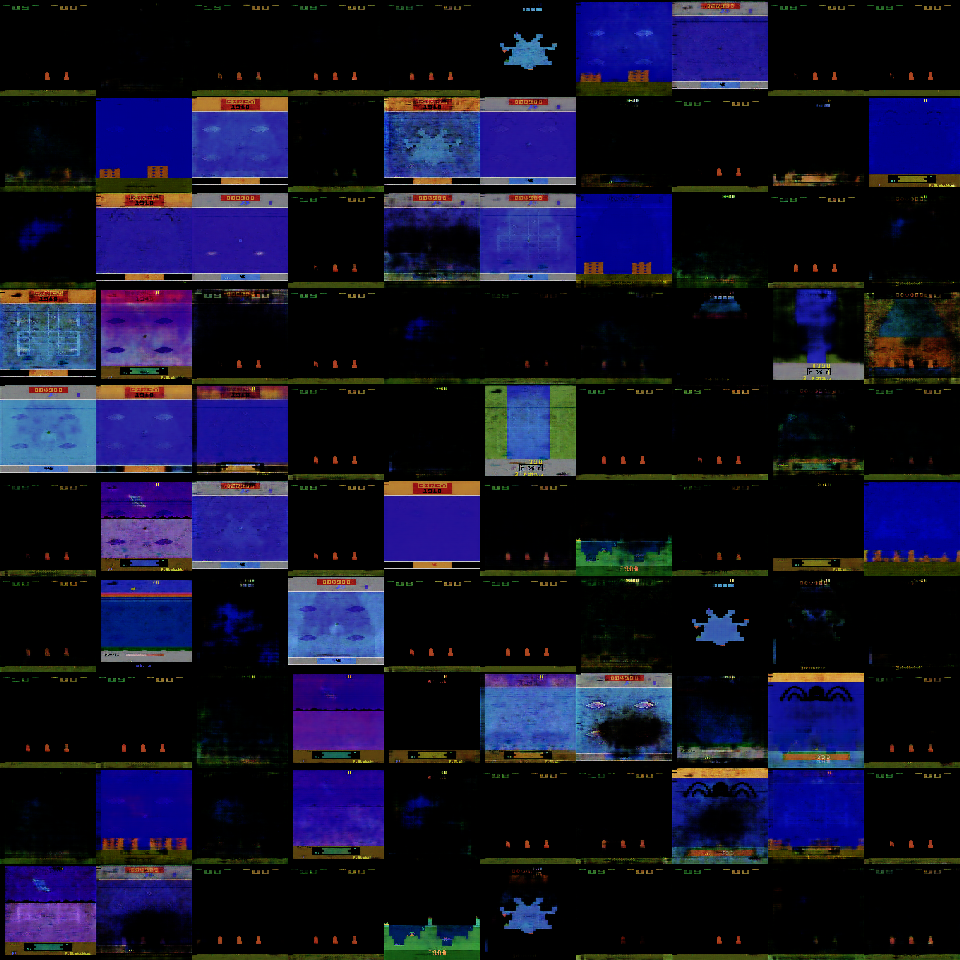
\includegraphics[width=0.8\linewidth]{withoutConditioning.png}
  \caption{Random reconstructions of Atari games using the trained VLAE without conditional instance normalization. In these reconstructions, one could see mode collapse and mixing up of the games. Compare to Figure \ref{fig:vlae}.}
  \label{fig:vlae-cond}
\end{figure}

\begin{table}
  \caption{Parameters for the Rainbow implementation}
  \label{tab:paramRAIN}
  \centering
  \begin{tabular}{ll}
    \toprule
    Parameter Description & Parameter Value\\
    \midrule
    Max episode length & 108,000\\
    Number of states processed at a time & 4\\
    Network hidden size & 512\\
    Initial standard deviation of noisy layers & 0.1\\
    Discretized size of value distribution & 51\\
    Replay memory capacity & 1,000,000\\
    Prioritized experience replay exponent & 0.5\\
    Minimum of value distribution & -10\\
    Maximum of value distribution & 10\\
    Frequency of sampling from memory & 4\\
    Initial prioritized experience replay importance sampling weight & 0.4\\
    Number of steps for multi-step return & 3\\
    Discount & 0.99\\
    Number of steps after which to update target network & 32,000 \\
    Reward clipping & 1\\
    Learning rate & 0.0000625\\
    Batch size & 32\\
    Number of steps before training starts & 80,000\\
    Number of evaluation episodes to average over & 10 \\
    Number of transitions to use for validating Q & 500 \\
    \bottomrule
  \end{tabular}
\end{table}

\begin{figure}
  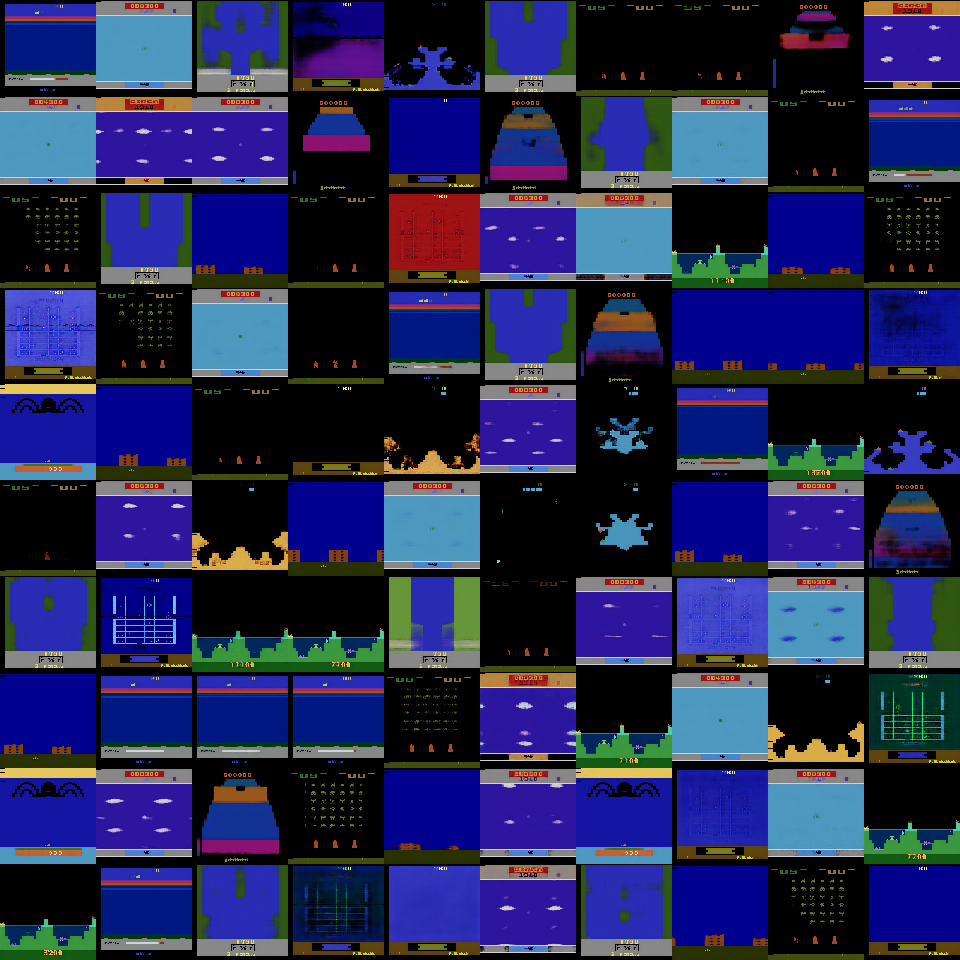
\includegraphics[width=0.8\linewidth]{epoch287.png}
  \caption{Random reconstructions of Atari games using the trained VLAE without coordinate convolutions. In these reconstructions, one could see mode collapse (the backgrounds are there, but no ships or other changing details). Compare to Figure \ref{fig:vlae}.}
  \label{fig:vlae-cordconv}
\end{figure}
\end{document}
